\subsection{Monte Carlo  Resolutions}
\label{sec:res_mctruth}
%
The jet \pt resolution derived from generator-level MC information   
information in the simulation, serves as a benchmark for the measurements 
of the jet resolution in collision data samples, 
using the methods introduced above and discussed in the following sections.

\begin{figure}[t]
\centering
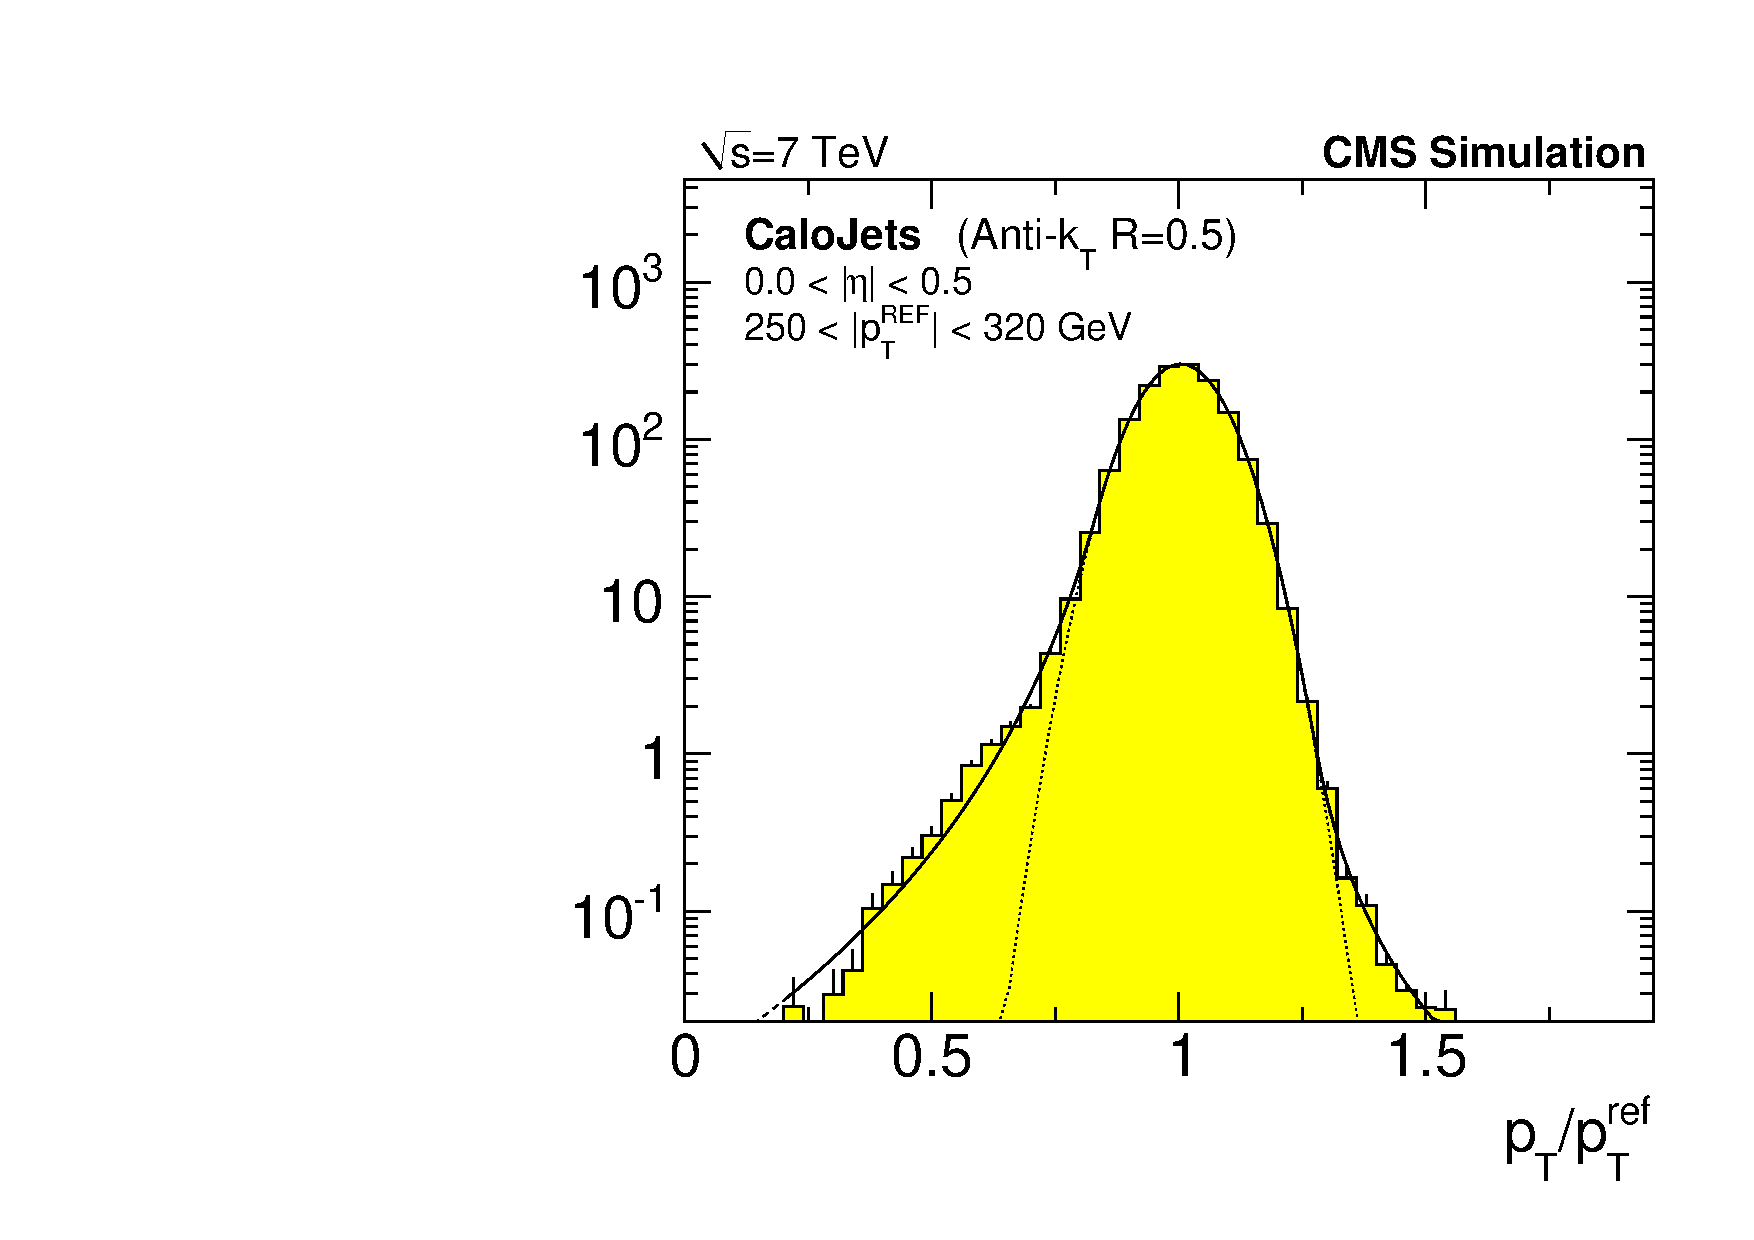
\includegraphics[width=0.49\textwidth]{Figures/JER/figs/res_mctruth/fit-example}
\caption{Distribution of the simulated CALO jet response, $\pt^{reco}/\pt^{gen}$, in a particular $|\eta|$ and $\pt^{gen}$ range. Fit examples with a Gaussian and a double-sided Crystal-Ball function are shown.
}
\label{fig:fit-example}
\end{figure}

The measurement of the jet \pt resolution in the simulation is performed using {\sc pythia} QCD dijet
events. The MC particle jets are matched geometrically to the reconstructed jets (CALO, JPT, or PF) by requiring
their distance in $\eta-\phi$ space to be $\Delta R < \Delta R_{Max}$.

The jet \pt response is defined as the ratio $\pt^{reco}/\pt^{gen}$
where $\pt^{reco}$ and $\pt^{gen}$ refer to the transverse momenta  
of the reconstructed jet and its matched reference MC particle jet respectively.

The width of the jet \pt response distribution, in a given $|\eta|$ and
$\pt^{gen}$ bin, is interpreted as the generator-level MC jet \pt 
resolution.  Figure~\ref{fig:fit-example} shows an example of 
$\pt^{reco}/\pt^{gen}$ distribution for CALO jets
in $|\eta|<0.5$ and with $250<\pt^{gen}<320\GeV$.

